\documentclass{beamer}
\usepackage[finnish]{babel}
\usepackage[T1]{fontenc}
\usepackage[utf8]{inputenc}
\usetheme{Warsaw}
\title[Data-assimilaatio kitkamallissa]{Data-assimilaatio kitkamallissa}
\author{Tom Gustafsson}
\date{5. syyskuuta 2012}
\begin{document}

\begin{frame}
\titlepage
\end{frame}

\begin{frame}{Ongelma}

\begin{itemize}
\item Lähtökohtana: Onnistuuko huonosti tunnettujen parametrien ennustaminen elastisesta kitkamallista data-assimilaation tarjoamien keinojen avulla?
\end{itemize}

\begin{figure}
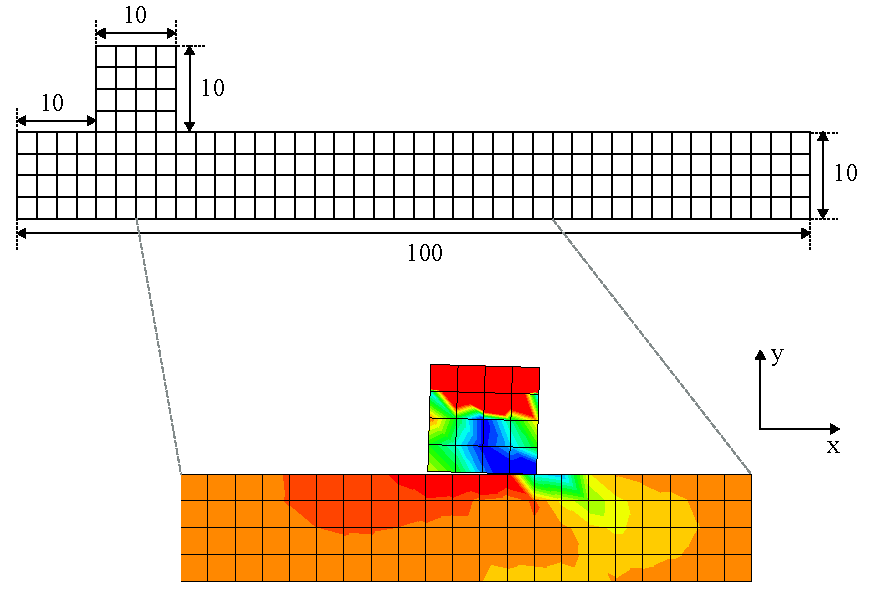
\includegraphics[width=8cm]{fretting_mesh.pdf}
\end{figure}

\end{frame}

\begin{frame}{Malli, 2D}

\begin{itemize}
\item Alkutila: Painin, laatta
\item Reunaehdot
\end{itemize}

\begin{figure}
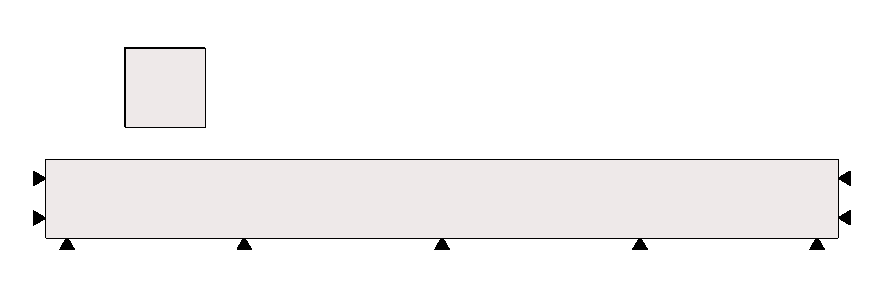
\includegraphics[width=10cm]{fretting_geom.pdf}
\end{figure}

\begin{itemize}
\item Abaqus/Standard 6.12-1
\end{itemize}

\end{frame}

\begin{frame}{Simulaation vaiheet}

\begin{itemize}
\item Vaihe 1: 5 kN voima
\end{itemize}

\begin{figure}
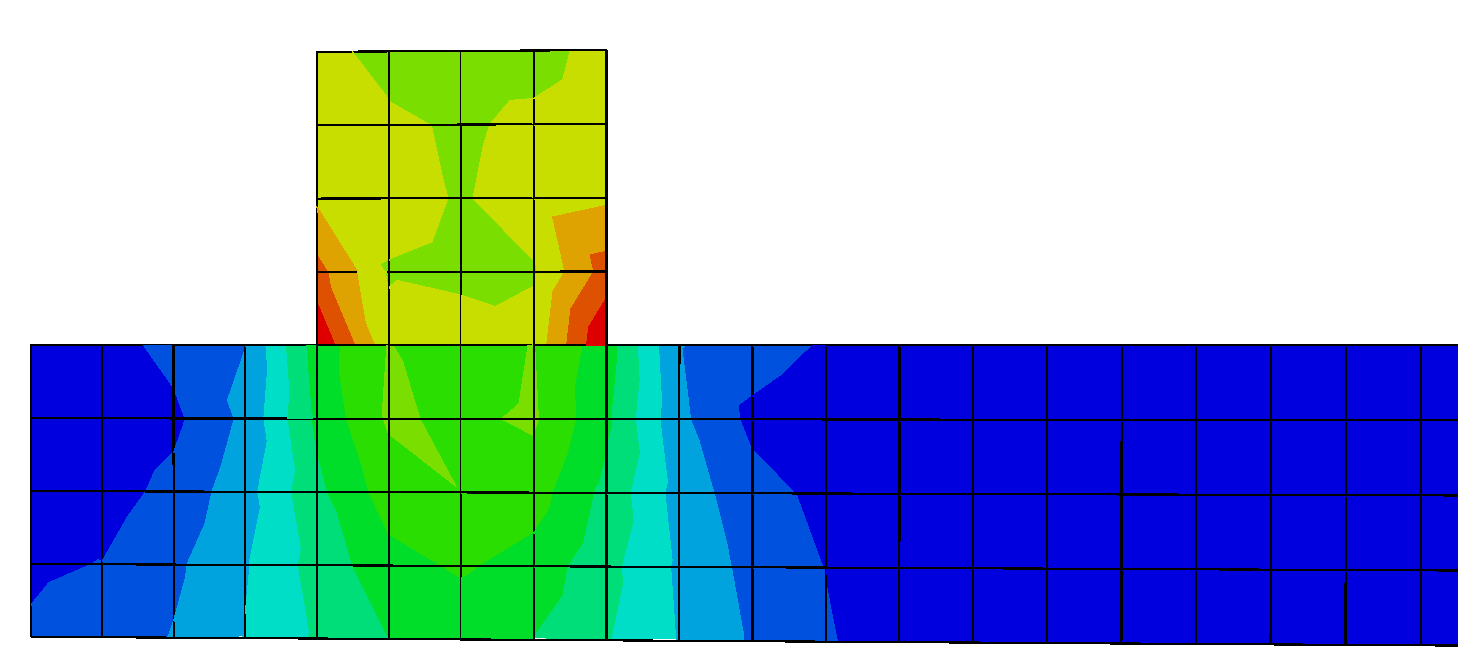
\includegraphics[width=9cm]{mises.pdf}
\end{figure}

\begin{itemize}
\item Vaihe 2: Yläreunan siirto 70 cm oikealle
\end{itemize}

\end{frame}

\begin{frame}{Simulaation vaiheet: Yläreunan siirtymä}

\begin{itemize}
\item Siirto reunaehdolla, ns. "hidas siirtymä"
\end{itemize}

\begin{figure}
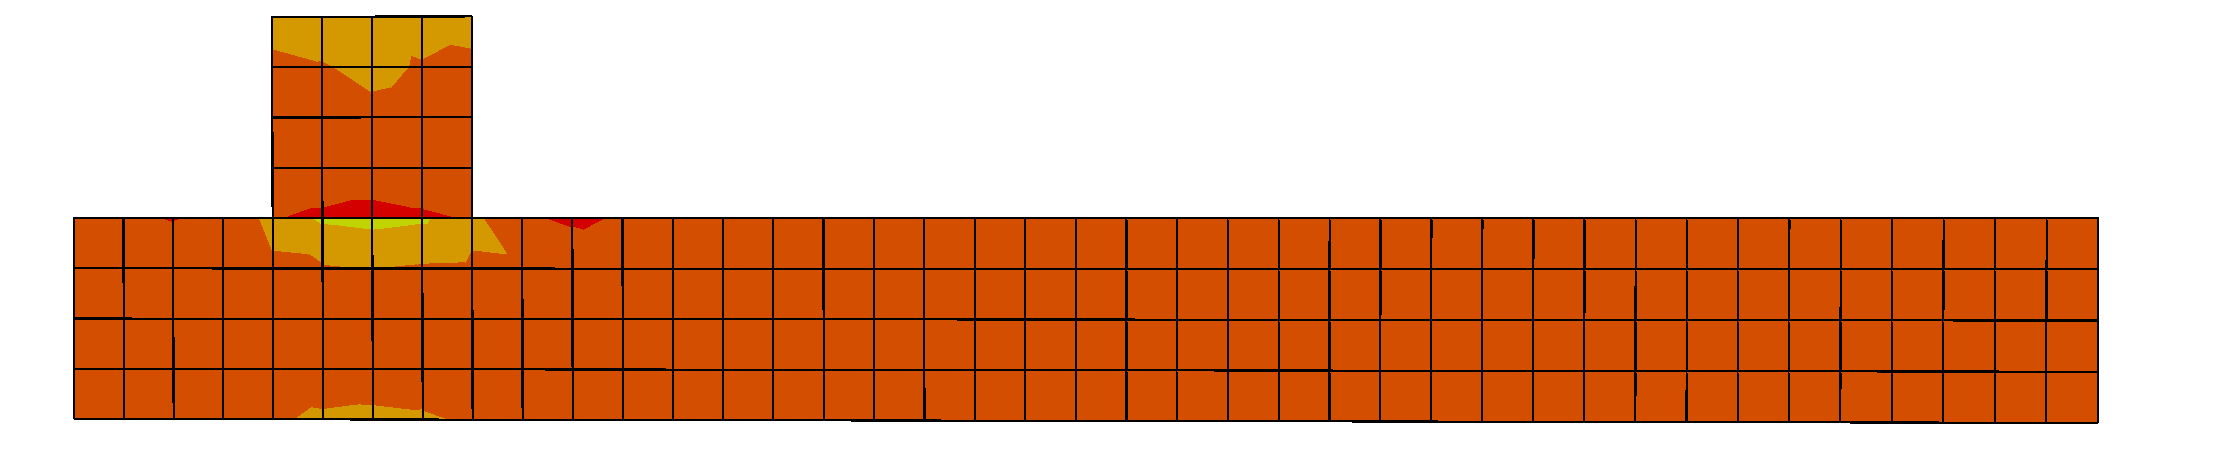
\includegraphics[width=10cm]{anim1.pdf}\\
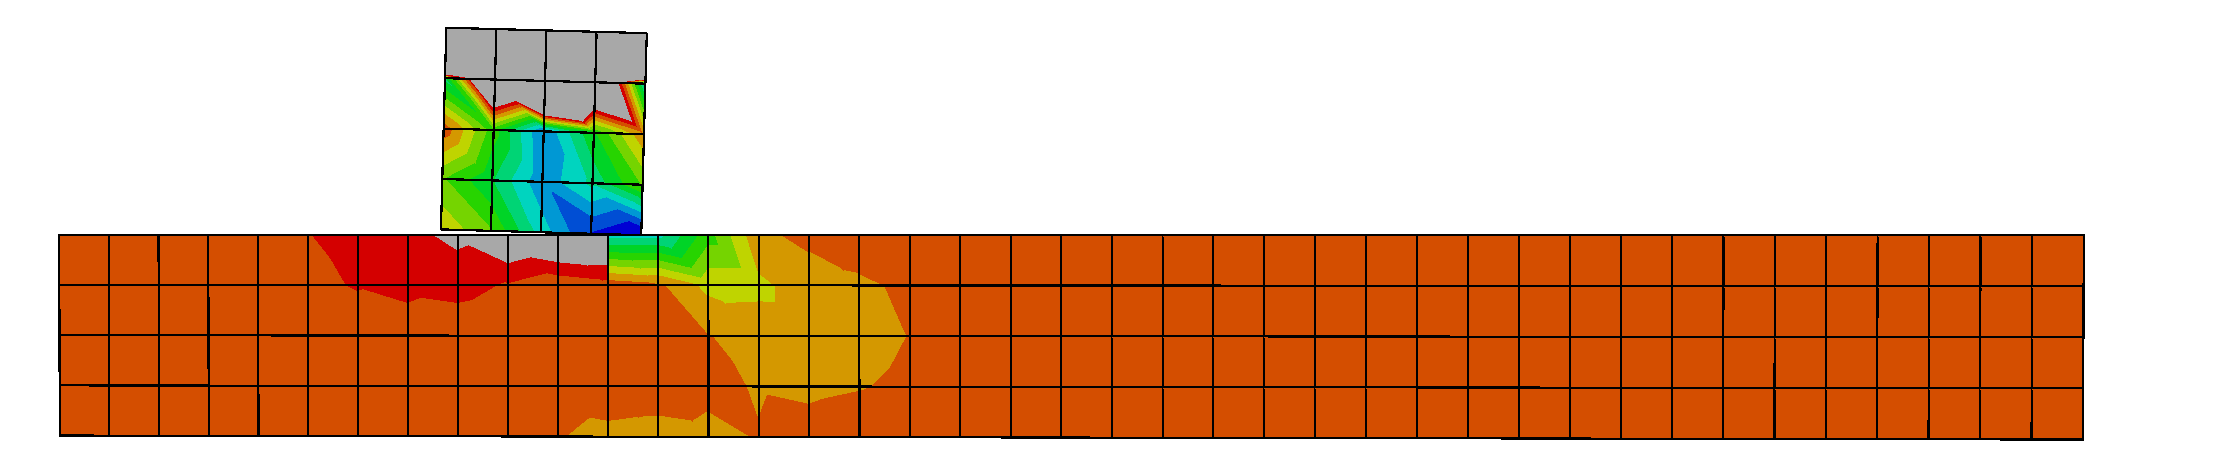
\includegraphics[width=10cm]{anim2.pdf}
\end{figure}

\end{frame}

\begin{frame}{Simulaation vaiheet: Yläreunan siirtymä 2}

\begin{figure}
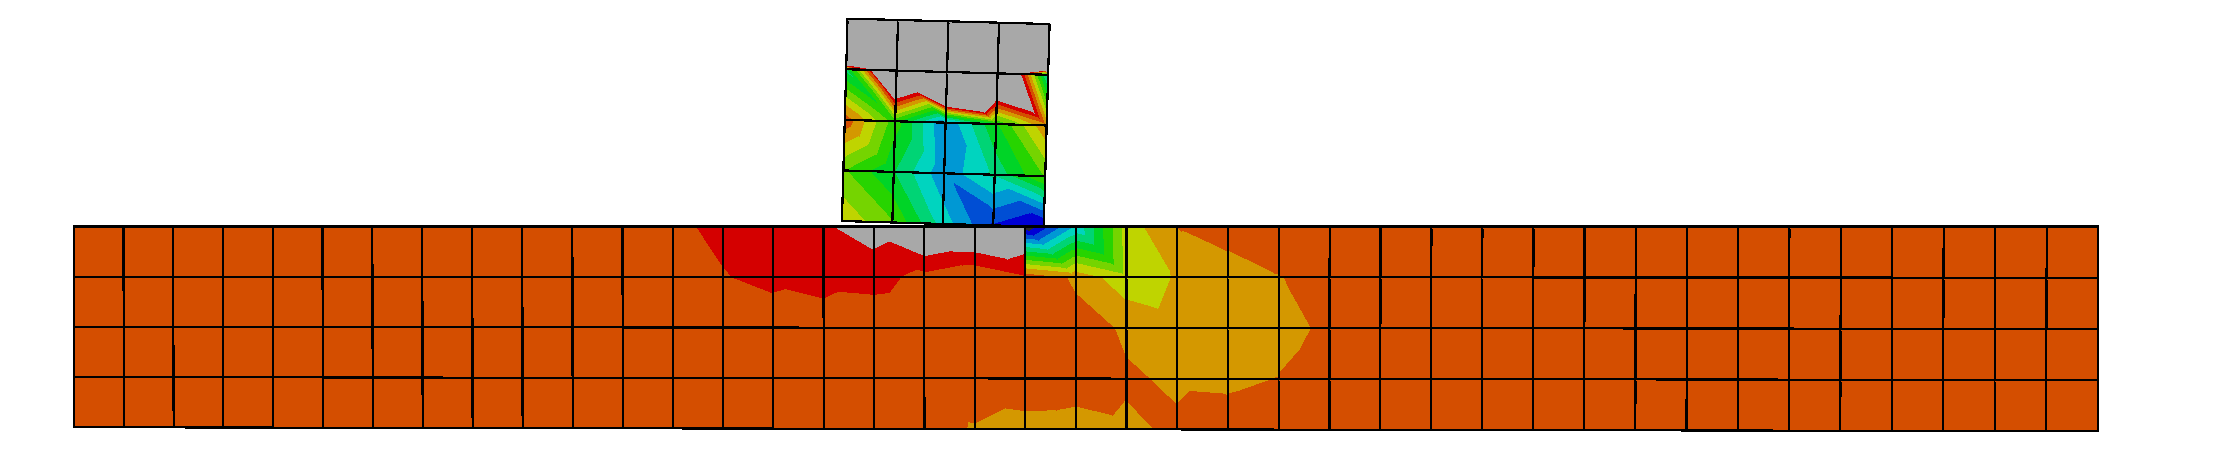
\includegraphics[width=10cm]{anim3.pdf}\\
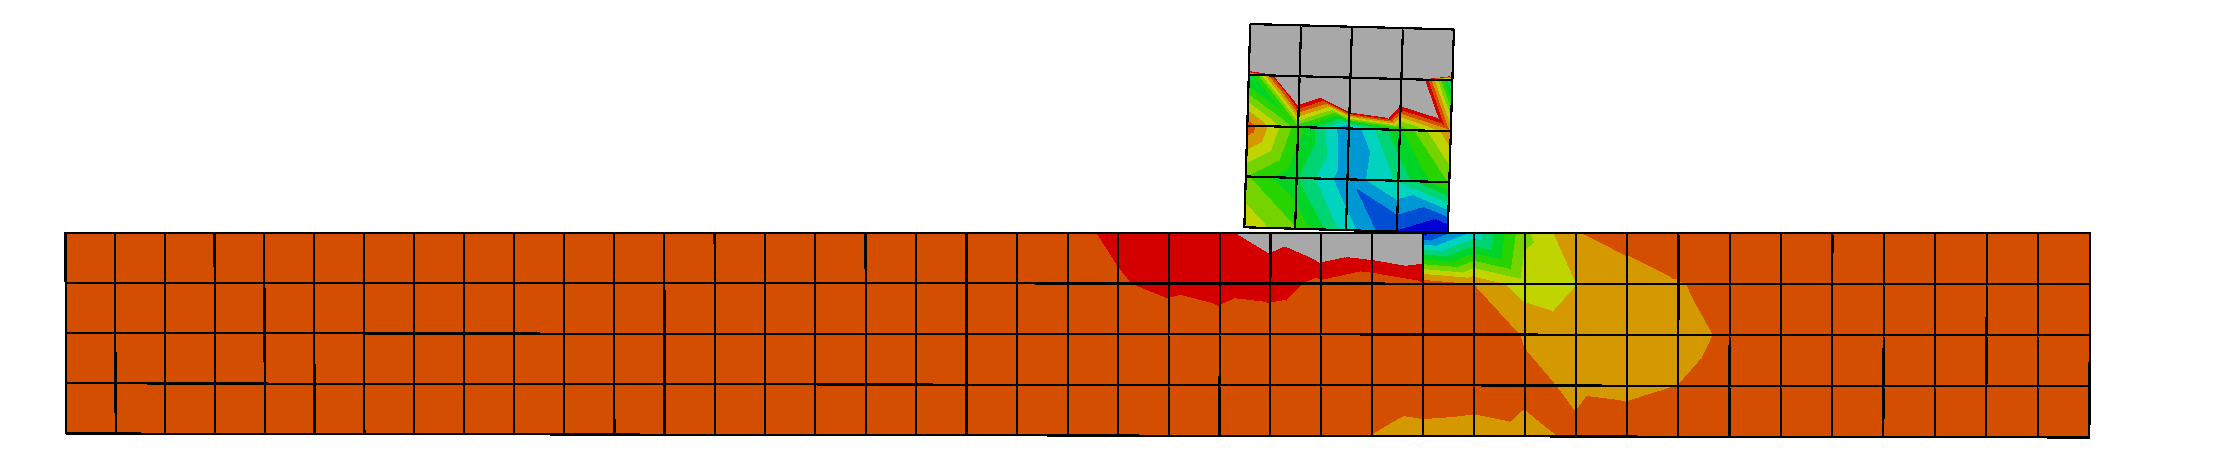
\includegraphics[width=10cm]{anim4.pdf}\\
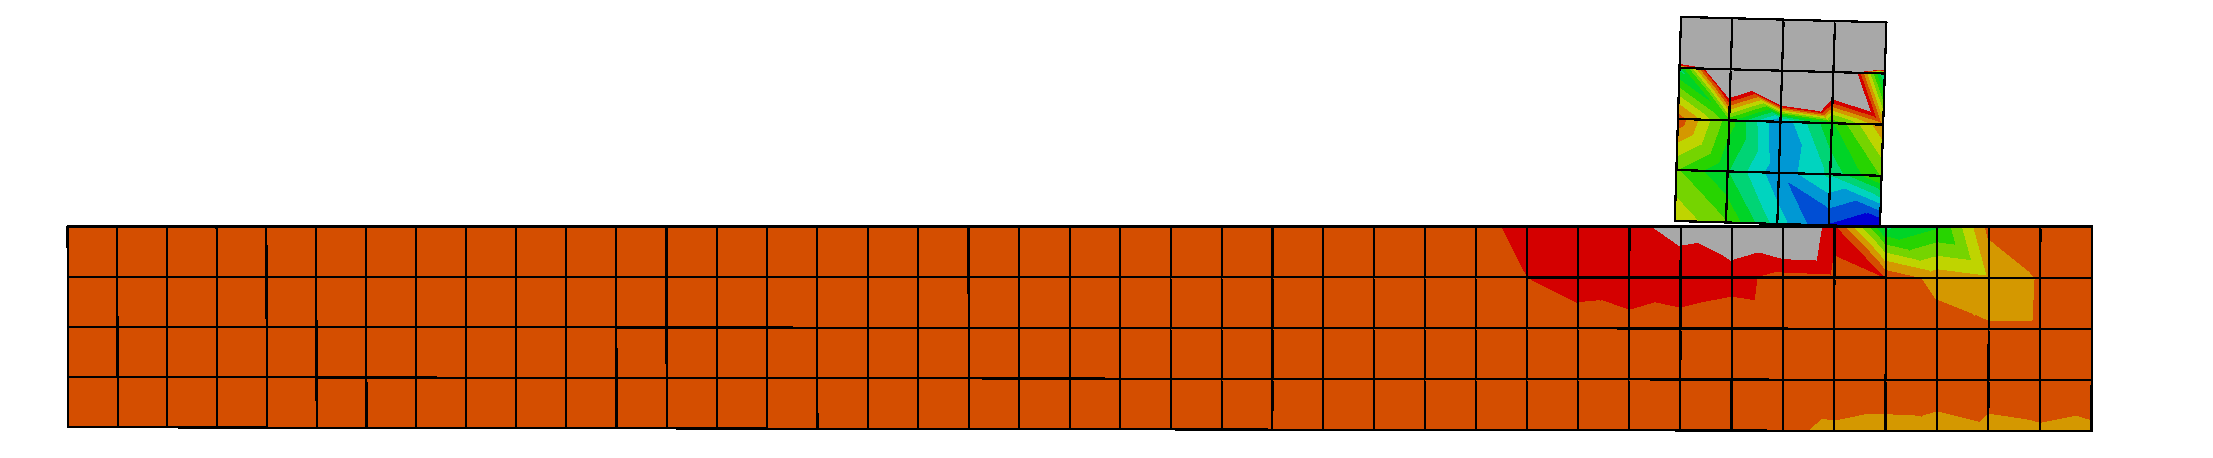
\includegraphics[width=10cm]{anim5.pdf}
\end{figure}

\end{frame}

\begin{frame}{Inversio-ongelma}

\begin{itemize}
\item Pyritään esimoimaan kitkakerroin $\mu$
\item Prioritietona $x$-suuntaiset jännitykset mittapisteissä\\($\sim$ venymäliuskamittaus)
\end{itemize}

\begin{figure}
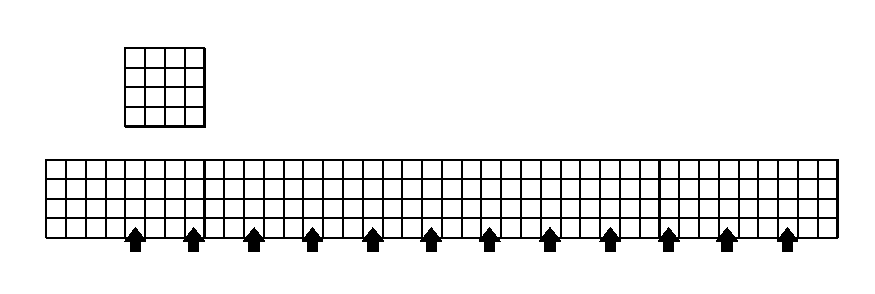
\includegraphics[width=10cm]{fretting_geom_meas.pdf}
\end{figure}

\begin{itemize}
\item Mittadata synteettistä
\end{itemize}

\end{frame}

\begin{frame}{Synteettisen mittadatan generointi}

\begin{itemize}
\item Minimoidaan inversiorikosta $\rightarrow$ mittadata tiheämmästä verkosta
\end{itemize}

\begin{figure}
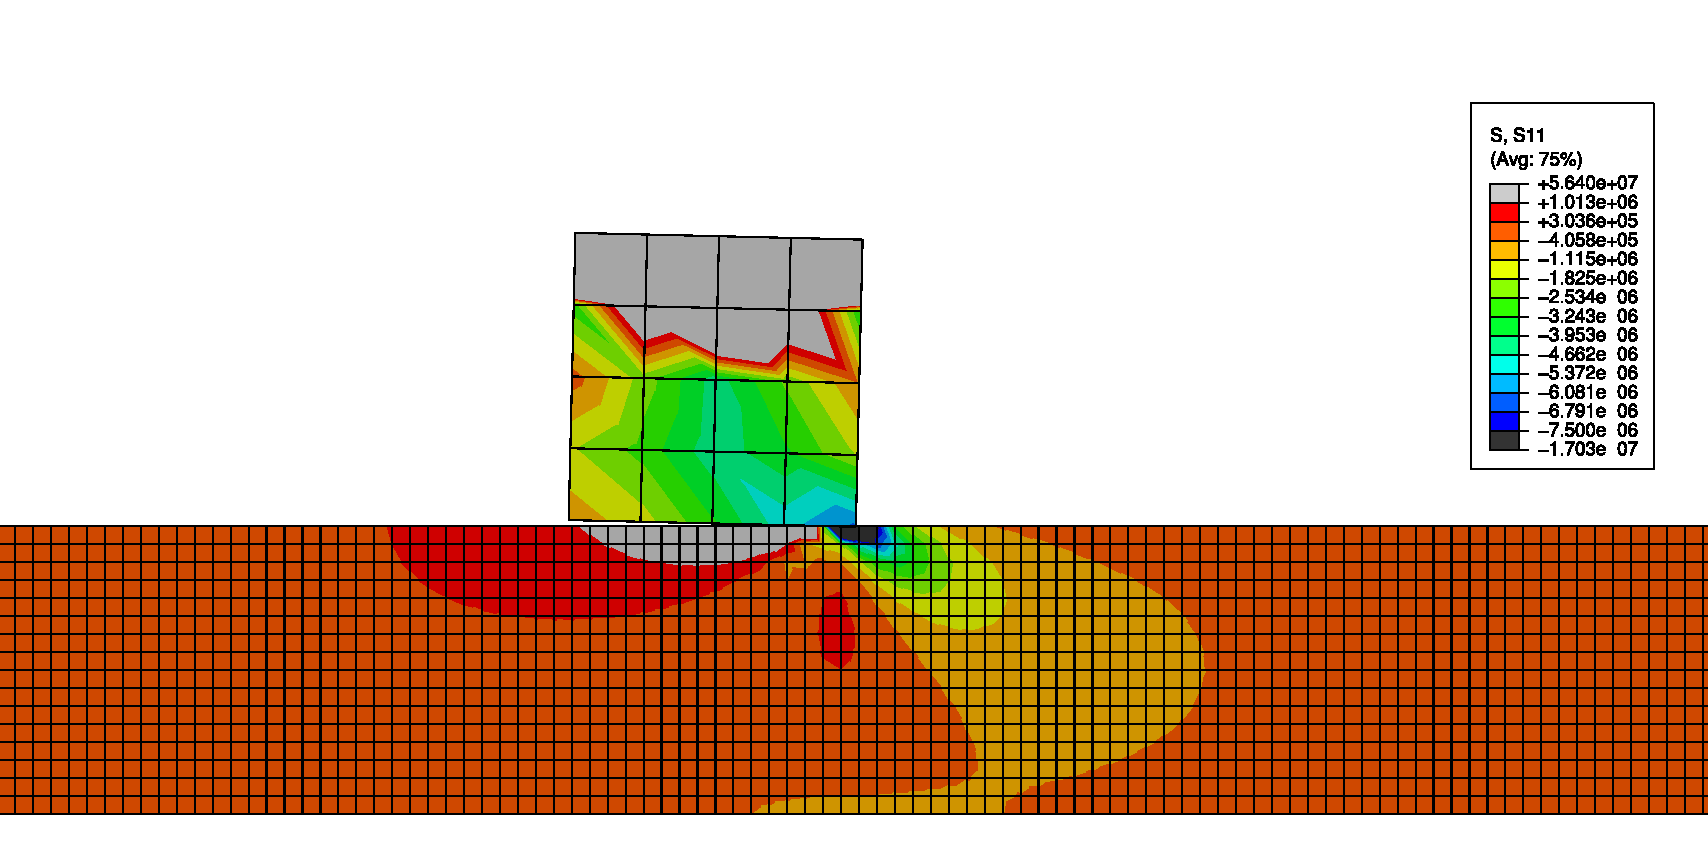
\includegraphics[width=10cm]{finer_mesh.pdf}
\end{figure}

\end{frame}

\begin{frame}{Synteettisen mittadatan generointi 2}

\begin{figure}
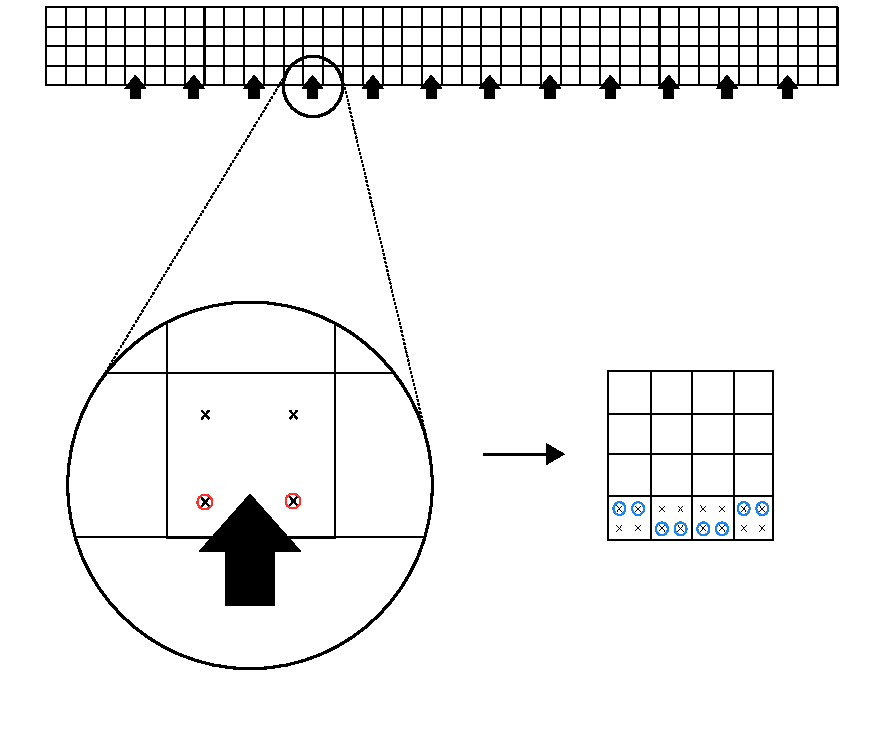
\includegraphics[width=10cm]{fretting_meas_tarkempi.pdf}
\end{figure}

\end{frame}

\end{document}
